\subsection*{Pochodne, monotoniczność i~ekstrema funkcji}
\subsubsection*{Zadanie~7.3.}
\begin{itemize}
    \item[f)]
        \begin{gather*}
            f\pars{x} = \frac{x^2 - 2x + 4}{x - 2} \qquad x \in \real \setminus \set{2}\\
            \begin{split}
                f'\pars{x}
                    &= \frac{\pars{x^2 - 2x + 4}'\pars{x - 2} - \pars{x^2 - 2x + 4}\pars{x - 2}'}{\pars{x - 2}^2}
                    = \frac{\pars{2x - 2}\pars{x - 2} - x^2 + 2x - 4}{\pars{x - 2}^2}\\
                    &= \frac{2x^2 - 6x + 4 - x^2 + 2x - 4}{\pars{x - 2}^2}
                    = \frac{x^2 - 4x}{\pars{x - 2}^2}
                    = \frac{x\pars{x - 4}}{\pars{x - 2}^2}
            \end{split}
        \end{gather*}
        Mianownik jest zawsze nieujemny, więc o~znaku pochodnej decyduje licznik:
        \begin{gather*}
            \upparabola{0}{4}\\
            \tag{\(1\)} \forall x \in \open{-\infty}{0}\colon f'\pars{x} > 0 \label{2020_10_21:7_3:f:first_increase}\\
            \tag{\(2\)} f'\pars{0} = 0 \label{2020_10_21:7_3:f:first_zero}\\
            \tag{\(3\)} \forall x \in \open{0}{4}\colon f'\pars{x} < 0 \label{2020_10_21:7_3:f:decrease}\\
            \tag{\(4\)} f'\pars{4} = 0 \label{2020_10_21:7_3:f:second_zero}\\
            \tag{\(5\)} \forall x \in \open{4}{+\infty}\colon f'\pars{x} > 0 \label{2020_10_21:7_3:f:second_increase}
        \end{gather*}
        Co z~tego wynika:
        \begin{description}
            \item \(\mbox{(\ref{2020_10_21:7_3:f:first_increase})} \implies\) funkcja \(f\) jest rosnąca w~przedziale \(\open{-\infty}{0}\)
            \item \(\mbox{(\ref{2020_10_21:7_3:f:first_increase})} \land \mbox{(\ref{2020_10_21:7_3:f:first_zero})} \land \mbox{(\ref{2020_10_21:7_3:f:decrease})} \implies\) funkcja \(f\) ma maksimum lokalne w~punkcie \(x = 0\):
                \begin{equation*}
                    f\pars{0} = \frac{4}{-2} = -2
                \end{equation*}
            \item \(\mbox{(\ref{2020_10_21:7_3:f:decrease})} \implies\) funkcja \(f\) jest malejąca w~przedziale \(\open{0}{4}\)
            \item \(\mbox{(\ref{2020_10_21:7_3:f:decrease})} \land \mbox{(\ref{2020_10_21:7_3:f:second_zero})} \land \mbox{(\ref{2020_10_21:7_3:f:second_increase})} \implies\) funkcja \(f\) ma minimum lokalne w~punkcie \(x = 4\):
                \begin{equation*}
                    f\pars{4} = \frac{16 - 8 + 4}{2} = 6
                \end{equation*}
                \item \(\mbox{(\ref{2020_10_21:7_3:f:second_increase})} \implies\) funkcja \(f\) jest rosnąca w~przedziale \(\open{4}{+\infty}\)
        \end{description}
    \item[k)]
        \begin{gather*}
            f\pars{x} = x\sqrt{4 - x} \qquad x \in \rightclosed{-\infty}{4}\\
            \begin{split}
                f'\pars{x}
                    &= \pars{x}'\pars{\sqrt{4 - x}} + x\pars{\sqrt{4 - x}}'
                    = 1 \cdot \sqrt{4 - x} - \frac{x}{2\sqrt{4 - x}}
                    = \frac{8 - 2x}{2\sqrt{4 - x}} - \frac{x}{2\sqrt{4 - x}}\\
                    &= \frac{8 - 3x}{2\sqrt{4 - x}} \qquad x \in \open{-\infty}{4}
            \end{split}
        \end{gather*}
        Mianownik jest zawsze nieujemny, więc o~znaku pochodnej decyduje licznik.
        \begin{gather*}
            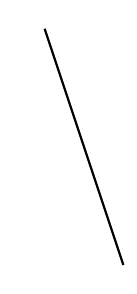
\begin{tikzpicture}
                \drawvec (0, 0) -- (4, 0) node[below]{\(x\)};
                \draw[thick] (2, 2) -- (3, -1);
                \fillpoint*{8/3, 0}[\(\frac{8}{3}\)][above right];
            \end{tikzpicture}
            \tag{\(1\)} \forall x \in \open{-\infty}{\frac{8}{3}}\colon f'\pars{x} > 0 \label{2020_10_21:7_3:k:increase}\\
            \tag{\(2\)} f'\pars{\frac{8}{3}} = 0 \label{2020_10_21:7_3:k:zero}\\
            \tag{\(3\)} \forall x \in \open{\frac{8}{3}}{4}\colon f'\pars{x} < 0 \label{2020_10_21:7_3:k:decrease}
        \end{gather*}
        Co z~tego wynika:
        \begin{description}
            \item \(\mbox{(\ref{2020_10_21:7_3:k:increase})} \implies\) funkcja \(f\) jest rosnąca w~przedziale \(\open{-\infty}{\frac{8}{3}}\)
            \item \(\mbox{(\ref{2020_10_21:7_3:k:increase})} \land \mbox{(\ref{2020_10_21:7_3:k:zero})} \land \mbox{(\ref{2020_10_21:7_3:k:decrease})} \implies\) funkcja \(f\) ma maksimum lokalne w~punkcie \(x = \frac{8}{3}\):
                \begin{equation*}
                    f\pars{\frac{8}{3}} = \frac{8}{3} \cdot \sqrt{\frac{12}{3} \cdot \frac{8}{4}} = \frac{8}{3} \cdot \sqrt{\frac{4}{3}} = \frac{16\sqrt{3}}{9}
                \end{equation*}
            \item \(\mbox{(\ref{2020_10_21:7_3:k:decrease})} \implies\) funkcja \(f\) jest malejąca w~przedziale \(\open{\frac{8}{3}}{4}\)
        \end{description}
        Zauważmy, że z~dziedziny pochodnej w~stosunku do dziedziny funkcji początkowej wypadł jeden punkt \(x = 4\). Styczna do wykresu w~tym miejscu jest pionowa, co oznacza że może tam być ekstremum. Rzeczywiście:
        \begin{gather*}
            f\pars{4} = 0\\
            \forall x \in \open{\frac{8}{3}}{4}\colon f\pars{x} = x\sqrt{4 - x} > 0
        \end{gather*}
        Zatem w~punkcie \(x = 4\) funkcja \(f\) ma minimum lokalne \(f\pars{4} = 0\).
    \item[\(\ell\))]
        \begin{gather*}
            f\pars{x} = x^2\sqrt{9 - x^2} \qquad x \in \closed{-3}{3}\\
            f'\pars{x} = \pars{x^2}'\pars{\sqrt{9 - x^2}} + x^2\pars{\sqrt{9 - x^2}}'
                = 2x\sqrt{9 - x^2} - \frac{x^3}{\sqrt{9 - x^2}}
                = \frac{18x - 3x^3}{\sqrt{9 - x^2}} \qquad x \in \open{-3}{3}
        \end{gather*}
        Mianownik jest zawsze nieujemny, więc o~znaku pochodnej decyduje licznik:
        \begin{gather*}
            18x - 3x^3 = 3\pars{6x - x^2} = 3x\pars{6 - x^2}\\
            
\begin{tikzpicture}
                \drawvec (-4, 0) -- (4, 0) node[below]{\(x\)};
                \draw[thick, domain=-3:3] plot (\x, {0.05 * \x * (6 - \x*\x)});
                \fillpoint*{0, 0}[\(0\)][above left];
                \fillpoint*{\fpeval{sqrt(6)}, 0}[\(\sqrt{6}\)][below left];
                \fillpoint*{-\fpeval{sqrt(6)}, 0}[\(-\sqrt{6}\)][below left];
            \end{tikzpicture}\\
            \tag{\(1\)} \forall x \in \open{-3}{-\sqrt{6}}\colon f'\pars{x} > 0 \label{2020_10_21:7_3:l:first_increase}\\
            \tag{\(2\)} f'\pars{-\sqrt{6}} = 0 \label{2020_10_21:7_3:l:first_zero}\\
            \tag{\(3\)} \forall x \in \open{-\sqrt{6}}{0}\colon f'\pars{x} < 0 \label{2020_10_21:7_3:l:first_decrease}\\
            \tag{\(4\)} f'\pars{0} = 0 \label{2020_10_21:7_3:l:second_zero}\\
            \tag{\(5\)} \forall x \in \open{0}{\sqrt{6}}\colon f'\pars{x} > 0 \label{2020_10_21:7_3:l:second_increase}\\
            \tag{\(6\)} f'\pars{\sqrt{6}} = 0 \label{2020_10_21:7_3:l:third_zero}\\
            \tag{\(7\)} \forall x \in \open{\sqrt{6}}{3}\colon f'\pars{x} < 0 \label{2020_10_21:7_3:l:second_decrease}
        \end{gather*}
        Co z~tego wynika:
        \begin{description}
            \item \(\mbox{(\ref{2020_10_21:7_3:l:first_increase})} \implies\) funkcja \(f\) jest rosnąca w~przedziale \(\open{-3}{-\sqrt{6}}\)
            \item \(\mbox{(\ref{2020_10_21:7_3:l:first_increase})} \land \mbox{(\ref{2020_10_21:7_3:l:first_zero})} \land \mbox{(\ref{2020_10_21:7_3:l:first_decrease})} \implies\) funkcja \(f\) ma maksimum lokalne w~punkcie \(x = -\sqrt{6}\):
                \begin{equation*}
                    f\pars{-\sqrt{6}} = 6\sqrt{3}
                \end{equation*}
            \item \(\mbox{(\ref{2020_10_21:7_3:l:first_decrease})} \implies\) funkcja \(f\) jest malejąca w~przedziale \(\open{-\sqrt{6}}{0}\)
            \item \(\mbox{(\ref{2020_10_21:7_3:l:first_decrease})} \land \mbox{(\ref{2020_10_21:7_3:l:second_zero})} \land \mbox{(\ref{2020_10_21:7_3:l:second_increase})} \implies\) funkcja \(f\) ma minimum lokalne w~punkcie \(x = 0\):
                \begin{equation*}
                    f\pars{0} = 0
                \end{equation*}
            \item \(\mbox{(\ref{2020_10_21:7_3:l:second_increase})} \implies\) funkcja \(f\) jest rosnąca w~przedziale \(\open{0}{\sqrt{6}}\)
            \item \(\mbox{(\ref{2020_10_21:7_3:l:second_increase})} \land \mbox{(\ref{2020_10_21:7_3:l:third_zero})} \land \mbox{(\ref{2020_10_21:7_3:l:second_decrease})} \implies\) funkcja \(f\) ma maksimum lokalne w~punkcie \(x = \sqrt{6}\):
                \begin{equation*}
                    f\pars{\sqrt{6}} = 6\sqrt{3}
                \end{equation*}
            \item \(\mbox{(\ref{2020_10_21:7_3:l:second_decrease})} \implies\) funkcja \(f\) jest malejąca w~przedziale \(\open{\sqrt{6}}{3}\)
        \end{description}
        Ponadto trzeba zauważyć, że względem dziedziny funkcji początkowej, z~dziedziny pochodnej wypadły punkty \(x = -3\) i~\(x = 3\). W~tych punktach styczna do wykresu funkcji \(f\) jest pionowa. Mogą tam być więc ekstrema. Rzeczywiście:
        \begin{gather*}
            f\pars{-3} = 0\\
            \forall x \in \open{-3}{-\sqrt{6}}\colon f'\pars{x} = x^2\sqrt{9 - x^2} > 0
        \end{gather*}
        Zatem w~punkcie \(x = -3\) funkcja \(f\) ma minimum lokalne \(f\pars{-3} = 0\). Ponadto
        \begin{gather*}
            f\pars{3} = 0\\
            \forall x \in \open{\sqrt{6}}{3}\colon f'\pars{x} = x^2\sqrt{9 - x^2} > 0
        \end{gather*}
        Zatem w~punkcie \(x = 3\) funkcja \(f\) ma minimum lokalne \(f\pars{3} = 0\).
\end{itemize}
\subsubsection*{Zadanie~7.7.}
\begin{itemize}
    \item[b)]
        \begin{gather*}
            f\pars{x} = 2x + \sin x \qquad x \in \real\\
            f'\pars{x} = 2 + \cos x\\
            -1 \leq \cos x \leq 1\\
            1 \leq 2 + \cos x \leq 3
        \end{gather*}
        Skoro pochodna zawsze jest dodatnia w~zbiorze \(\real\), to znaczy że funkcja \(f\) jest rosnąca w~tym zbiorze.
        \qed
\end{itemize}
\subsubsection*{Zadanie~7.9.}
\begin{equation*}
    \forall x \in \open{0}{\frac{\pi}{2}}\colon \sin x + \tan x > 2x
\end{equation*}
Zdefiniujmy funkcję
\begin{equation*}
    f\pars{x} = \sin x + \tan x - 2x
\end{equation*}
i~zauważmy, że jest ciągła jako suma funkcji ciągłych. Jest też określona dla \(x = 0\):
\begin{equation*}
    f\pars{0} = 0
\end{equation*}
Zbadajmy jej pochodną:
\begin{equation*}
    f'\pars{x} = \cos x + \frac{1}{\cos^2x} - 2
\end{equation*}
Również jest ona ciągła jako suma funkcji ciągłych oraz jest określona dla \(x = 0\):
\begin{equation*}
    f'\pars{0} = 1 + \frac{1}{1} - 2 = 0
\end{equation*}
Zbadajmy z~kolei jej pochodną:
\begin{equation*}
    f''\pars{x} = -\sin x - \frac{-2\sin x\cos x}{\cos^4x} = -\sin x + \frac{2\sin x\cos x}{\cos^4x} = -\sin x + \frac{2\sin x}{\cos^3x}
\end{equation*}
Dla \(x \in \open{0}{\frac{\pi}{2}}\) zachodzi \(0 < \cos x < 1\), czyli \(0 < \cos^3x < 1\), oraz \(\sin x > 0\) więc:
\begin{equation*}
    \forall x \in \open{0}{\frac{\pi}{2}}\colon f''\pars{x} = -\sin x + \frac{2\sin x}{\cos^3x} > -\sin x + 2\sin x = \sin x > 0
\end{equation*}
Skoro \(f''\) jest dodatnia w~przedziale \(\open{0}{\frac{\pi}{2}}\) oraz \(f'\) jest ciągła i~dla \(x = 0\) przyjmuje wartość \(0\), to znaczy, że \(f'\) jest rosnąca od \(0\), czyli dodatnia w~tym przedziale. Dodatniość \(f'\) oznacza z~kolei, że skoro \(f\) jest ciągła i~dla \(x = 0\) przyjmuje wartość \(0\), to znaczy, że \(f\) jest rosnąca od \(0\), czyli dodatnia w~tym przedziale. Zatem
\begin{gather*}
    \sin x + \tan x - 2x > 0\\
    \sin x + \tan x > 2x
\end{gather*}
\qed
\subsubsection*{Zadanie~7.10.}
\begin{enumerate}[label={\alph*)}]
    \item
        \begin{description}
            \item[Założenia:] \(x > -1 \land x \neq 0 \land \pars{p < 0 \lor p > 1}\)
            \item[Teza:] \(\pars{1 + x}^p > 1 + px\)
        \end{description}
        Rozważmy przypadki:
        \begin{proofcases}
            \item \(x > 0 \land p > 1\)
                \begin{gather*}
                    1 + x > 1\\
                    \pars{1 + x}^{p - 1} > 1
                \end{gather*}
                Zdefniujmy funkcję
                \begin{equation*}
                    f\pars{x} = \pars{1 + x}^p - px - 1
                \end{equation*}
                Zauważmy, że jest ona ciągła (jako suma funkcji ciągłych) i~określona dla \(x = 0\):
                \begin{equation*}
                    f\pars{0} = \pars{1}^p - 1 = 1 - 1 = 0
                \end{equation*}
                Policzmy pochodną:
                \begin{gather*}
                    f'\pars{x} = p\pars{1 + x}^p - p = \overbrace{p}^{> 0}\overbrace{\pars{\pars{1 + x}^{p - 1} - 1}}^{> 0 \text{ dla } x > 0}\\
                    \forall x > 0\colon f'\pars{x} > 0
                \end{gather*}
                Dla \(x > 0\) pochodna jest większa od \(0\), czyli funkcja jest rosnąca. Skoro funkcja jest ciągła, \(f\pars{0} = 0\) i~jest rosnąca, to znaczy, że zawsze jest dodatnia:
                \begin{gather*}
                    \pars{1 + x}^p - px - 1 > 0\\
                    \pars{1 + x}^p > px + 1
                \end{gather*}
                co kończy dowód dla tego przypadku.
            \item \(x > 0 \land p < 0\)
                \begin{gather*}
                    1 + x > 1\\
                    0 < \pars{1 + x}^{p - 1} < 1
                \end{gather*}
                Zdefniujmy funkcję
                \begin{equation*}
                    f\pars{x} = \pars{1 + x}^p - px - 1
                \end{equation*}
                Zauważmy, że jest ona ciągła (jako suma funkcji ciągłych) i~określona dla \(x = 0\):
                \begin{equation*}
                    f\pars{0} = \pars{1}^p - 1 = 1 - 1 = 0
                \end{equation*}
                Policzmy pochodną:
                \begin{gather*}
                    f'\pars{x} = p\pars{1 + x}^p - p = \overbrace{p}^{< 0}\overbrace{\pars{\pars{1 + x}^{p - 1} - 1}}^{< 0 \text{ dla } x > 0}\\
                    \forall x > 0\colon f'\pars{x} > 0
                \end{gather*}
                Dla \(x > 0\) pochodna jest większa od \(0\), czyli funkcja jest rosnąca. Skoro funkcja jest ciągła, \(f\pars{0} = 0\) i~jest rosnąca, to znaczy, że zawsze jest dodatnia:
                \begin{gather*}
                    \pars{1 + x}^p - px - 1 > 0\\
                    \pars{1 + x}^p > px + 1
                \end{gather*}
                co kończy dowód dla tego przypadku.
            \item \(x \in \open{-1}{0} \land p > 1\)
                Zdefniujmy funkcję
                \begin{equation*}
                    f\pars{x} = \pars{1 + x}^p - px - 1
                \end{equation*}
                Zauważmy, że jest ona ciągła (jako suma funkcji ciągłych) i~określona dla \(x = -1\):
                \begin{equation*}
                    f\pars{-1} = \pars{0}^p + p - 1 = p - 1 > 0
                \end{equation*}
                Policzmy pochodną:
                \begin{gather*}
                    f'\pars{x} = p\pars{1 + x}^p - p = \overbrace{p}^{> 0}\overbrace{\pars{\pars{1 + x}^{p - 1} - 1}}^{< 0 \text{ dla } x \in \open{-1}{0}}\\
                    \forall x \in \open{-1}{0}\colon f'\pars{x} < 0
                \end{gather*}
                Funkcja jest malejąca, a~w zerze przyjmuje wartość \(0\). Zatem musi być zawsze większa od zero dla \(x \in \open{-1}{0}\).
                \begin{gather*}
                    \pars{1 + x}^p - px - 1 > 0\\
                    \pars{1 + x}^p > px + 1
                \end{gather*}
                co kończy dowód dla tego przypadku.
            \item \(x \in \open{-1}{0} \land p < 0\)
                Zdefniujmy funkcję
                \begin{equation*}
                    f\pars{x} = \pars{1 + x}^p - px - 1
                \end{equation*}
                Zauważmy, że jest ona ciągła (jako suma funkcji ciągłych) i~określona dla \(x = -1\):
                \begin{equation*}
                    f\pars{-1} = \pars{0}^p + p - 1 = p - 1 > 0
                \end{equation*}
                Policzmy pochodną:
                \begin{gather*}
                    f'\pars{x} = p\pars{1 + x}^p - p = \overbrace{p}^{< 0}\overbrace{\pars{\pars{1 + x}^{p - 1} - 1}}^{> 0 \text{ dla } x \in \open{-1}{0}}\\
                    \forall x \in \open{-1}{0}\colon f'\pars{x} < 0
                \end{gather*}
                Funkcja jest malejąca, a~w zerze przyjmuje wartość \(0\). Zatem musi być zawsze większa od zero dla \(x \in \open{-1}{0}\).
                \begin{gather*}
                    \pars{1 + x}^p - px - 1 > 0\\
                    \pars{1 + x}^p > px + 1
                \end{gather*}
                co kończy dowód dla tego przypadku.
        \end{proofcases}
        \qed
\end{enumerate}
\subsubsection*{Zadanie~7.12.}
\begin{itemize}
    \item[a)]
        \begin{equation*}
            \cos x = \frac{\pi}{2} - x
        \end{equation*}
        Konstruujemy funkcję:
        \begin{gather*}
            f\pars{x} = \cos x + x - \frac{\pi}{2}\\
            f'\pars{x} = -\sin x + 1\\
            f'\pars{x} = 0 \iff x = \frac{\pi}{2} + 2k\pi \qquad k \in \integer\\
            f'\pars{x} \geq 0 \qquad x \in \real
        \end{gather*}
        Funkcja jest niemalejąca, ale skoro te punkty, w~których pochodna się zeruje, są izolowane, to możemy to wzmocnić: funkcja jest rosnąca! Zatem jeśli zgadniemy jedno rozwiązanie, to jest ono jedyne. Trywialnie zgadujemy jedno rozwiązanie \(x = \frac{\pi}{2}\) i~wiemy, że jest ono jedyne.
\end{itemize}
\subsubsection*{Zadanie~8.13.}
\begin{itemize}
    \item[e)]
        \begin{gather*}
            f\pars{x} = \frac{1}{x^3 - 6x^2 + 9x + 20} \qquad x \in \closed{-1}{5}\\
            f'\pars{x}
                = -\frac{\pars{x^3 - 6x^2 + 9x + 20}'}{\pars{x^3 - 6x^2 + 9x + 20}^2}
                = -\frac{3x^2 - 12x + 9}{\pars{x^3 - 6x^2 + 9x + 20}^2}
        \end{gather*}
        Mianownik jest zawsze nieujemny, więc znak pochodnej zależy tylko od licznika:
        \begin{gather*}
            -\pars{3x^2 - 12x + 9}\\
            -\pars{x^2 - 4x + 3}\\
            -\pars{x - 1}\pars{x - 3}\\
            \downparabola{1}{3}\\
            \tag{\(1\)} \forall x \in \open{-1}{1}\colon f'\pars{x} < 0 \label{2020_10_21:8_13:e:first_decrease}\\
            \tag{\(2\)} f'\pars{1} = 0 \label{2020_10_21:8_13:e:first_zero}\\
            \tag{\(3\)} \forall x \in \open{1}{3}\colon f'\pars{x} > 0 \label{2020_10_21:8_13:e:increase}\\
            \tag{\(4\)} f'\pars{3} = 0 \label{2020_10_21:8_13:e:second_zero}\\
            \tag{\(5\)} \forall x \in \open{3}{5}\colon f'\pars{x} < 0 \label{2020_10_21:8_13:e:second_decrease}
        \end{gather*}
        Co z~tego wynika:
        \begin{description}
            \item \(\mbox{(\ref{2020_10_21:8_13:e:first_decrease})} \implies\) funkcja \(f\) jest malejąca w~przedziale \(\open{-1}{1}\)
            \item \(\mbox{(\ref{2020_10_21:8_13:e:first_decrease})} \land \mbox{(\ref{2020_10_21:8_13:e:first_zero})} \land \mbox{(\ref{2020_10_21:8_13:e:increase})} \implies\) funkcja \(f\) ma minimum lokalne w~punkcie \(x = 1\):
                \begin{equation*}
                    f\pars{1} = \frac{1}{1 - 6 + 9 + 20} = \frac{1}{24}
                \end{equation*}
            \item \(\mbox{(\ref{2020_10_21:8_13:e:increase})} \implies\) funkcja \(f\) jest rosnąca w~przedziale \(\open{1}{3}\)
            \item \(\mbox{(\ref{2020_10_21:8_13:e:increase})} \land \mbox{(\ref{2020_10_21:8_13:e:second_zero})} \land \mbox{(\ref{2020_10_21:8_13:e:second_decrease})} \implies\) funkcja \(f\) ma maksimum lokalne w~punkcie \(x = 3\):
                \begin{equation*}
                    f\pars{3} = \frac{1}{27 - 54 + 27 + 20} = \frac{1}{20}
                \end{equation*}
            \item \(\mbox{(\ref{2020_10_21:8_13:e:second_decrease})} \implies\) funkcja \(f\) jest malejąca w~przedziale \(\open{3}{5}\)
        \end{description}
        Ponadto, skoro dziedzina funkcji jest domknięta i~funkcja jest malejąca przedziale \(\open{-1}{1}\), to w~punkcie \(x = -1\) jest maksimum lokalne:
        \begin{equation*}
            f\pars{-1} = \frac{1}{-1 - 6 - 9 + 20} = \frac{1}{4}
        \end{equation*}
        Podobnie, skoro funkcja jest malejąca w~przedziale
\end{itemize}
